% 2011 年湖南卷理科第 20 题：雨中移动的长方体。
% 来源 PDF：普通高考/2011/2011湖南理.pdf，SHA-256 09b67f1db8e6a280165cf8431211a968163c0d0f262a50068dd607607a9ec578。
% 原页：第 2 页第 2 栏上部，书页码 672。示意。
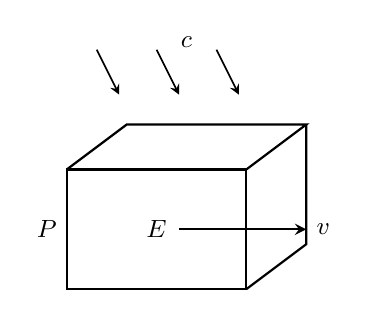
\begin{tikzpicture}[>=stealth, semithick, font=\small, scale=0.95]
  \draw[thick] (0,0)--(2.4,0)--(2.4,1.6)--(0,1.6)--cycle;
  \draw[thick] (0,1.6)--(0.8,2.2)--(3.2,2.2)--(2.4,1.6);
  \draw[thick] (2.4,0)--(3.2,0.6)--(3.2,2.2);
  \node at (1.2,0.8) {$E$};
  \draw[->, thick] (1.5,0.8)--(3.2,0.8) node[right] {$v$};
  \foreach \x in {0.4,1.2,2.0} \draw[->] (\x,3.2)--(\x+0.3,2.6);
  \node at (1.6,3.3) {$c$};
  \node[left] at (0,0.8) {$P$};
\end{tikzpicture}
